\documentclass{article}
\usepackage[polish]{babel}
\usepackage[a4paper, margin=2cm]{geometry}
\usepackage{graphicx}
\usepackage{polski}
\usepackage[utf8]{inputenc}
\usepackage{lettrine}
\usepackage{xcolor}
\usepackage[nodayofweek]{datetime}
\renewcommand{\familydefault}{\sfdefault}

\usepackage{biblatex}
\addbibresource{bibliography.bib}

\makeatletter
\renewcommand{\maketitle}{\bgroup\setlength{\parindent}{0pt}
\begin{flushleft}
\@title

\large{\textbf{   \@author}}

\large{\textbf{   \@date}}
\end{flushleft}\egroup
}
\makeatother

\title{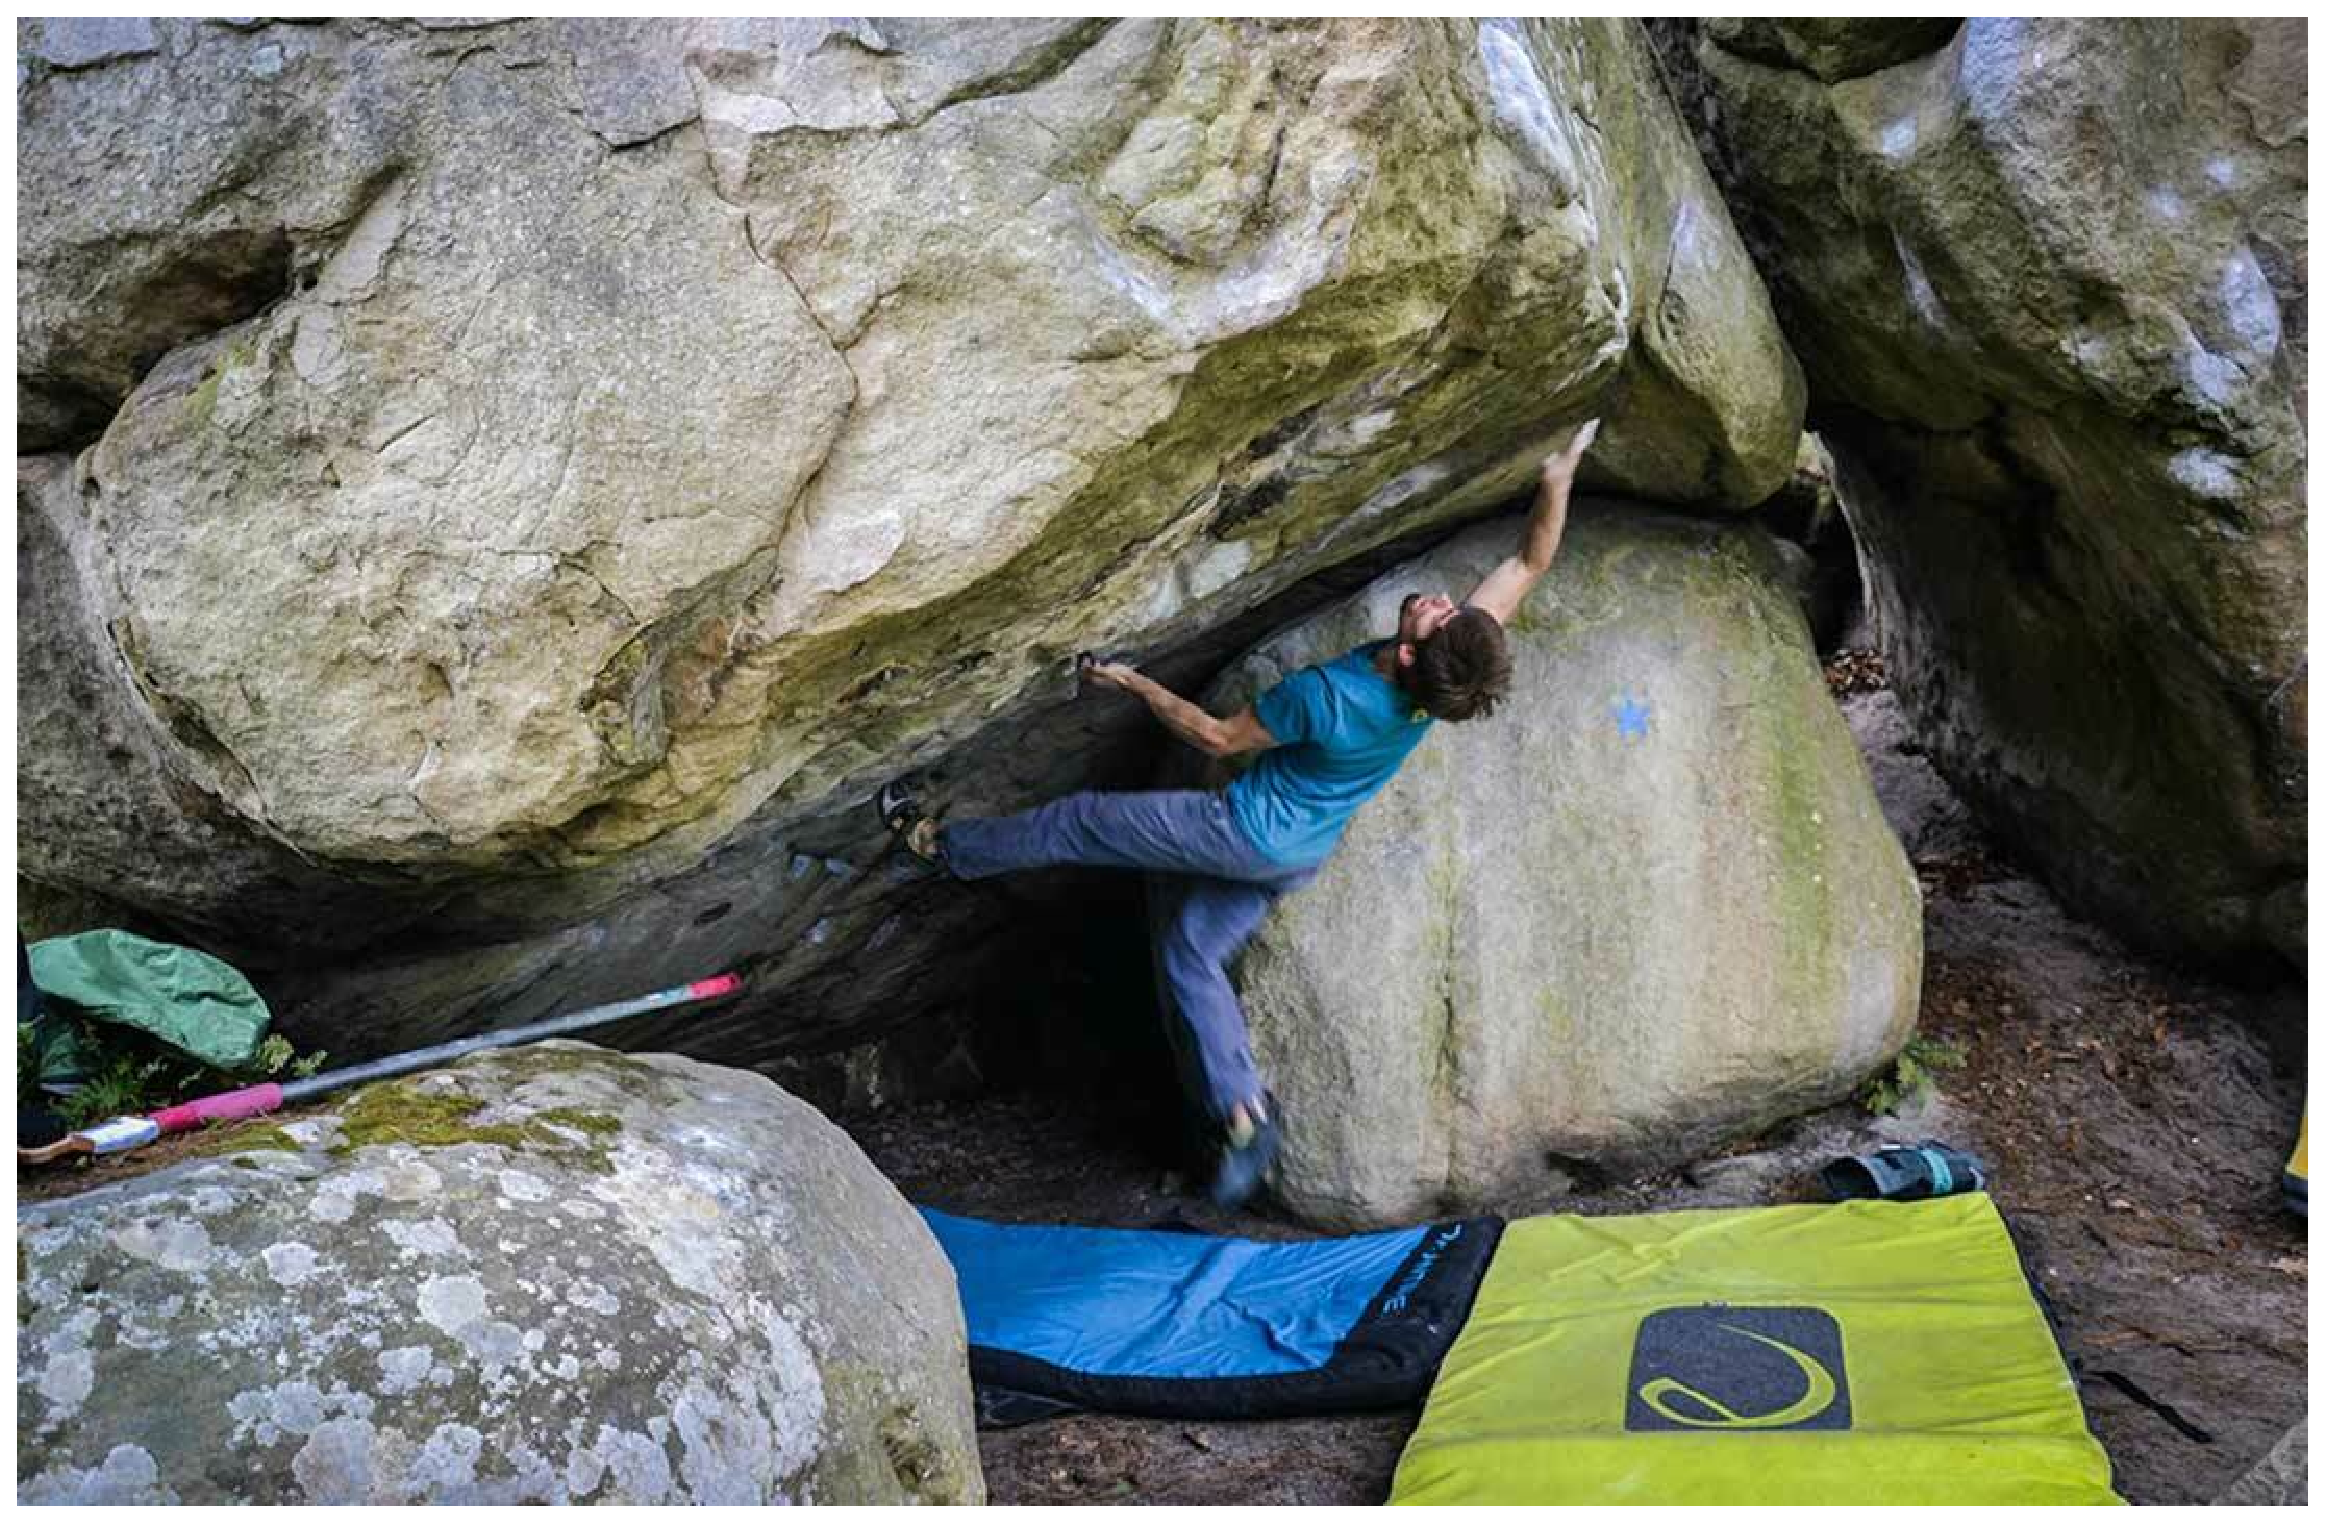
\includegraphics[width=\linewidth]{images/intro.eps}}
\author{Marcin Młynarczyk}
\newdate{date}{11}{6}{2020}
\date{\displaydate{date}}
\definecolor{blue}{cmyk}{.6,.28,0,.04}
\definecolor{lighter-blue}{cmyk}{.59,.14,0,.04}

\usepackage{sectsty}
\chapterfont{\color{blue}}
\sectionfont{\color{blue}}
\subsectionfont{\color{blue}}

\addto\captionspolish{
  \renewcommand{\contentsname}%
    {\color{blue}Spis treści}%
}

\begin{document}

\maketitle
\tableofcontents

\section{Wstęp}
\lettrine[lines=3]{B}{ouldering} staje się coraz popularniejszą formą aktywności fizycznej. Owy termin, w swojej angielskiej postaci, dość mocno zakorzenił się w polskim żargonie wspinaczkowym. Pojęcie \textit{bouldering} pochodzi z języka angielskiego, w którym oznacza \textit{głaz}. Zatem uprawianie boulderingu to w dosłownym tłumaczeniu "głazowanie", czyli wspinanie się na głazy. W języku polskim można się również spotkać z lekko spolszczoną wersją tego terminu - \textit{baldering}. W dużym uproszczeniu, i trochę żartobliwie, bouldering można zdefiniować jako "wchodzenie na kamyki od trudnej strony". W odróżnieniu od wspinaczki z liną, asekurację najczęściej stanowią tutaj materace rozłożone w potencjalnej strefie upadku. Z tego również powodu, jako obiekt wspinania obiera się tutaj z reguły wolnostojące głazy poniżej 6 m wysokości. Niemniej jednak, można spotkać od tej reguły wyjątki, np. boulder o nazwie \textit{Ambrosia} w Bishop, Colorado w USA posiada ponad 16 m wysokości.

\section{Historia}
\lettrine[lines=3]{S}{kupię} się na przedstawieniu światowej historii rozwoju omawianego w tej pracy sportu, jako że w dostępnych źródłach bardzo ciężko doszukać się informacji na temat polskiej historii boulderingu. Postaram się przytoczyć okoliczności powstania boulderingu, a następnie przejdę do jego obecnej sytuacji. 


\subsection{Początki}
\subsection{Obecnie}

\section{Znaczące osoby}
\subsection{John Gill}
\subsection{John Sherman}
\subsection{Fred Nicole}
\subsection{Ashima Shiraishi}
\subsection{Nalle Hukkataival}

\nocite{*}
\printbibliography

\end{document}
